\begin{figure}[ht]
  \centering
  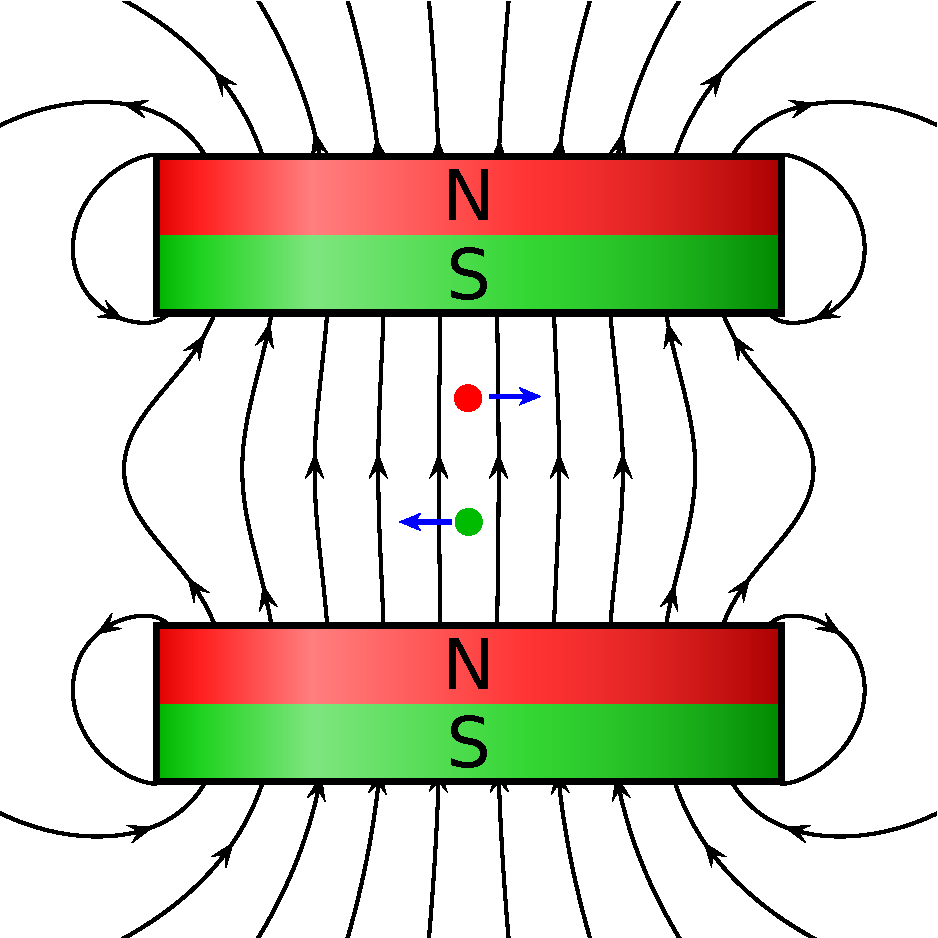
\includegraphics[trim={1cm 1cm 1cm 1cm}, clip, width=.6\textwidth]{uniform_gap}
  \caption{A representation of a pair of idealised cylindrical magnets in a
    dipole configuration. Two positively charged particles are shown as circles,
    the red particle is traveling out of the page, the green particle is
    traveling into the page. The forces experienced by each particle due to the
    magnetic field are shown as blue arrows.}
  \label{fig:dipole}
\end{figure}
